\subsubsection{Однополупериодные выпрямители, их свойства}

Однополупериодные выпрямители характеризуются тем, что пропускают только положительную (отрицательную) волну синусоидального тока.

\begin{center}
	\begin{figure}[h!]
		\center{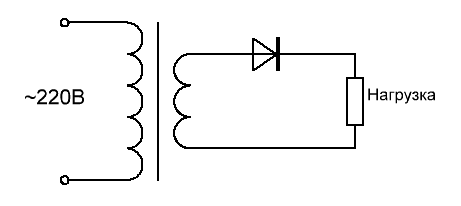
\includegraphics[scale=0.9]{1pp.png}}
		\caption{Схема элементарного 1 п/п выпрямителя}
	\end{figure}
\end{center} 

Среднее значение напряжение определяется как и в случае 2 п/п выпрямителя.

Выходное напряжение имеет следующее разложение в ряд Фурье:
\begin{equation}
U_{out} = \frac{U_m}{\pi} + \frac{U_m}{2} sin(\omega t) ...
\end{equation}
\begin{equation}
U_{mid} = \sqrt{2} \frac{U_{in}}{\pi}
\end{equation}
КПД:
\begin{equation}
\nu = \frac{I^2 R_n}{I^2 (R_n + r_d)}
\end{equation}